\subsection{Eigengesichter als Basis}
Im letzten Unterkapitel haben wir den Raum der Differenzgesichter eingeführt.
In diesem Unterkapitel wollen wir eine geeignete Basis dieses Unterraumes finden, nämlich die \textit{Eigengesichter}.
Um uns einige grundlegende Begriffe aus der linearen Algebra in Erinnerung zu rufen, betrachten wir folgende Aufgabe.
\begin{aufgabe}
	Betrachten Sie die Vektoren
	\begin{equation*}
		\vec v_1=\begin{pmatrix}
			\tfrac{3}{5} \\ \tfrac{4}{5} \\ 0
		\end{pmatrix},\quad
		\vec v_2=\begin{pmatrix}
			-\tfrac{4}{5} \\ \tfrac{3}{5} \\  0
		\end{pmatrix},\quad
		\vec v_3=\begin{pmatrix}
			0 \\ 0 \\  1
		\end{pmatrix},\quad
		\vec a=\begin{pmatrix}
			7 \\ 1 \\  4
		\end{pmatrix}.
	\end{equation*}
	\begin{enumerate}[label=(\alph*)]
		\item Die Vektoren $\vec v_1,\vec v_2,\vec v_3$ bilden eine orthonormale Basis von $\mathbb R^3$.
		Begründen Sie warum.
		\item Folglich gibt es genau eine Linearkombination
		\begin{equation*}
			\vec a=c_1\vec v_1+c_2\vec v_2+c_3\vec v_3.
		\end{equation*}
		Berechnen Sie die Koeffizienten $c_1,c_2,c_3$ dieser Linearkombination.
	\end{enumerate}
\end{aufgabe}
\begin{losung*}
	\phantom{text}
	\begin{enumerate}[label=(\alph*)]
		\item Die Vektoren $\vec v_1,\vec v_2,\vec v_3$ sind paarweise orthogonal, also
		\begin{equation*}
			\vec v_1\cdot\vec v_2= \tfrac{3}{5}\cdot\left(-\tfrac{4}{5}\right)+\tfrac{4}{5}\cdot\tfrac{3}{5}+0\cdot 0=0
		\end{equation*}
		und analog findet man $\vec v_1\cdot\vec v_3=0$ und $\vec v_2\cdot\vec v_3=0$.
		Insbesondere sind die Vektoren linear unabhängig.
		Da es drei an der Zahl sind, müssen Sie eine Basis von $\mathbb R^3$ sein.
		Zudem haben die Vektoren Länge Eins, das heisst
		\begin{equation*}
			\vec v_1\cdot\vec v_1= \left(\tfrac{3}{5}\right)^2+\left(\tfrac{4}{5}\right)^2+0^2=1.
		\end{equation*}
		Analog findet man $\vec v_2\cdot\vec v_2=1$ und $\vec v_3\cdot\vec v_3=1$.
		Damit ist diese Basis nicht nur orthogonal, sondern sogar orthonormal.
		\item Da unsere Basis orthonormal ist, kann man die Koeffizienten mit einem Skalarprodukt berechnen.
		Zum Beispiel findet man den Koeffizienten $c_1$ indem man auf beiden Seiten der Gleichung aus der Teilaufgabe das Skalarprodukt mit $v_1$ bildet
		\begin{equation*}
			\vec v_1\cdot\vec a=c_1\underbrace{\vec v_1\cdot\vec v_1}_{=1}+c_2\underbrace{\vec v_1\cdot\vec v_2}_{=0}+c_3\underbrace{\vec v_1\cdot\vec v_3}_{=0},
		\end{equation*}
		also $\vec v_1\cdot\vec a=c_1$.
		Analog erhält man $\vec v_2\cdot\vec a=c_2$ und $\vec v_3\cdot\vec a=c_3$.
		Diese Skalarprodukte berechnen sich zu
		\begin{equation*}
			c_1=5,\quad\quad c_2=-5,\quad\quad c_3=4.
		\end{equation*}
	\end{enumerate}
\end{losung*}

%Die Bilder $\vec a_1,\ldots,\vec a_K$ aus unserer Datenbank sind im Allgemeinen nicht paarweise orthogonal und nicht auf Länge 1 normiert.
Wir werden im Folgenden annehmen, dass die Anzahl der Bilder $K$ viel kleiner ist als die Anzahl der Pixel $M\cdot N$ der einzelnen Bilder.
Der Einfachheit halber nehmen wir zudem an, dass die Vektoren $\vec a_1,\ldots,\vec a_K$ linear unabhängig sind.
Diese bilden dann die Basis eines $K$-dimensionalen Unterraums von $\mathbb R^{M\cdot N}$.
Nun betrachten wir eine weitere Basis dieses Unterraumes, die \textit{Eigengesichter}.
Die Eigengesichter sind eine orthonormale Basis dieses Raumes, wir bezeichnen diese mit $\vec u_1,\dots,\vec u_K\in\mathbb R^{M\cdot N}$.
Diese Basis ist in vielerlei Hinsicht speziell, wie wir sehen werden.
Diese Vektoren können wir wieder als Bilder darstellen.
Das ist in Abbildung~\ref{fig:eigenfaces} gezeigt.
\begin{figure}[ht]
	\centering
	\begin{tabular}{cccccccc}
		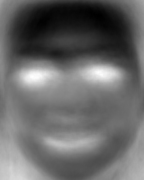
\includegraphics[width=0.1\textwidth]{images/eigenfaces/eigenface00} & 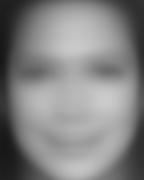
\includegraphics[width=0.1\textwidth]{images/eigenfaces/eigenface01} &
		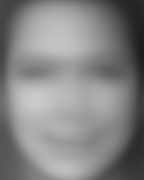
\includegraphics[width=0.1\textwidth]{images/eigenfaces/eigenface02} & 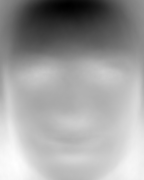
\includegraphics[width=0.1\textwidth]{images/eigenfaces/eigenface03} &
		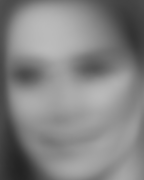
\includegraphics[width=0.1\textwidth]{images/eigenfaces/eigenface04} &
		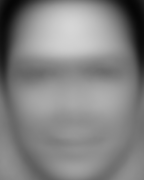
\includegraphics[width=0.1\textwidth]{images/eigenfaces/eigenface05} & 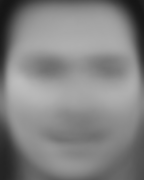
\includegraphics[width=0.1\textwidth]{images/eigenfaces/eigenface06} &
		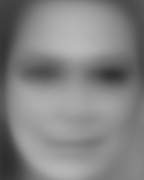
\includegraphics[width=0.1\textwidth]{images/eigenfaces/eigenface07} \\ 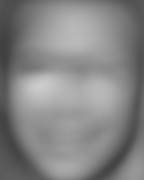
\includegraphics[width=0.1\textwidth]{images/eigenfaces/eigenface08} &
		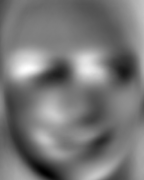
\includegraphics[width=0.1\textwidth]{images/eigenfaces/eigenface09} & 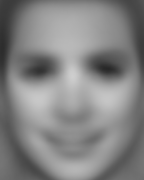
\includegraphics[width=0.1\textwidth]{images/eigenfaces/eigenface10} &
		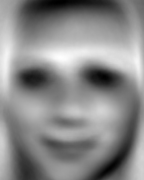
\includegraphics[width=0.1\textwidth]{images/eigenfaces/eigenface11} & 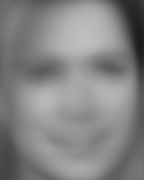
\includegraphics[width=0.1\textwidth]{images/eigenfaces/eigenface12} &
		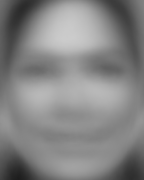
\includegraphics[width=0.1\textwidth]{images/eigenfaces/eigenface13} & 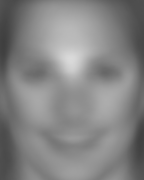
\includegraphics[width=0.1\textwidth]{images/eigenfaces/eigenface14} &
		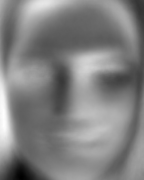
\includegraphics[width=0.1\textwidth]{images/eigenfaces/eigenface15} \\
	\end{tabular}
	\caption{Die ersten 16 Eigengesichter wurden wieder als Bild dargestellt.}
	\label{fig:eigenfaces}
\end{figure}

Wir betrachten nun die Mona Lisa von Leonardo da Vinci, ein Bild das nicht in unserer Datenbank ist.
Um dieses Bild in den Raum der Differenzgesichter zu verschieben, müssen wir noch das Durchschnittsgesicht $\vec m$ subtrahieren.
Das entstehende Differenzgesicht kann dann näherungsweise als Linearkombination der Basis $\vec a_1,\ldots,\vec a_K$ oder auch der Basis der Eigengesichter $\vec u_1,\ldots,\vec u_K$ dargestellt werden.
Letzteres ist in Abbildung~\ref{fig:eigen_basis} dargestellt.
\begin{figure}[ht]
	\centering
	\begin{tabular}{m{1.8cm} c c c c c m{2cm} c c c m{2cm} c c}
		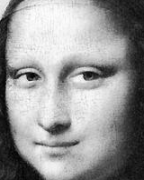
\includegraphics[width=0.1\textwidth]{images/eigenfaces/mona_lisa_original} &
		$-$ & $\vec m$ & $=$ & $c_1$ & $\cdot$ & 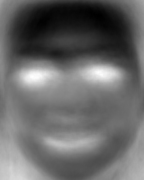
\includegraphics[width=0.1\textwidth]{images/eigenfaces/eigenface00}
		& $+$ & $c_2$ & $\cdot$ & 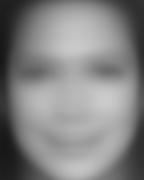
\includegraphics[width=0.1\textwidth]{images/eigenfaces/eigenface01} & $+$ & $\cdots$
	\end{tabular}
	\caption{Differenzgesicht der Mona Lisa als Linearkombination der Eigengesichter.}
	\label{fig:eigen_basis}
\end{figure}
\begin{aufgabe}
	Sei $\vec p\in\mathbb R^{M\cdot N}$ das Bild der Mona Lisa und $\vec u_1,\ldots,\vec u_K\in\mathbb R^{M\cdot N}$ die Eigengesichter.
	Berechnen Sie die Koeffizienten $c_1,\ldots,c_K$ der Linearkombination der Eigengesichter, also
	\begin{equation*}
		\vec p-\vec m=c_1\vec u_1+c_2\vec u_2+\ldots+c_K\vec u_K
	\end{equation*}
	wie in Abbildung~\ref{fig:eigen_basis} gezeigt.
	Das heisst, geben Sie die Koeffizienten in Termen von $\vec p, \vec m$ und den Eigengesichtern an.
\end{aufgabe}
\begin{losung*}
	Wie in der letzten Aufgabe verwenden wir, das die Eigengesichter orthonormal sind.
	Wir bilden das Skalarprodukt beider Seiten der obigen Gleichung mit $u_1$, also
	\begin{equation*}
		\vec u_1\cdot\left(\vec p-\vec m\right)=c_1\underbrace{\vec u_1\cdot\vec u_1}_{=1}+c_2\underbrace{\vec u_1\cdot\vec u_2}_{=0}+\ldots+c_K\underbrace{\vec u_1\cdot\vec u_K}_{=0}.
	\end{equation*}
	Wenn wir das auch noch mit $\vec u_2,\ldots,\vec u_K$ machen erhalten wir
	\begin{equation*}
		\vec u_k\cdot\left(\vec p-\vec m\right)=c_k,
	\end{equation*}
	für alle $k\in\{1,\ldots,K\}$.
\end{losung*}
Hat man die Koeffizienten der Linearkombination berechnet, so kann das Bild $\vec p$ der Mona Lisa wieder als Linearkombination der Eigengesichter darstellen
\begin{equation*}
	\vec p=\vec m+c_1\vec u_1+c_2\vec u_2+\ldots+c_Ku_K.
\end{equation*}
Das werden wir in der nächsten Aufgabe implementieren.
\begin{aufgabe} \label{aufg:compute_coefficients}
	Seien \texttt{p} und \texttt{m} Vektoren der Länge $M\cdot N$, wobei \texttt{p} ein Gesicht zeigt (z.B. das der Mona Lisa) und \texttt{m} das Durchschnittsgesicht ist.
	Sei zudem \texttt{u\_list} die Liste der Eigengesichter als Vektoren.
	Ergänzen Sie die Funktion \texttt{compute\_coefficients(p, m, u\_list)}, welche die Liste der Koeffizienten der Linearkombination aus Abbildung~\ref{fig:eigen_basis} zurück gibt.
	Um Ihre Lösung zu testen können Sie das Python Skript \texttt{basis\_expansion.py} laufen lassen, welches das Bild der Mona Lisa mit ihren Koeffizienten rekonstruiert.
	\textit{Hinweis:} Mit \texttt{np.dot(v,w)} lässt sich das Skalarprodukt zweier Vektoren \texttt{v} und \texttt{w} berechnen.
\end{aufgabe}
\begin{losung*}
	Die Lösung könnte zum Beispiel so aussehen.\\[0.5cm]
	\begin{minipage}{0.65\textwidth}
\begin{lstlisting}[style=python]
import numpy as np

def compute_coefficients(p, m, u_list):
	K = len(u_list)
	c_list = np.empty((K,))
	for c, u in zip(c_list, u_list):
		c = np.dot(u, p - m)
	return c_list
\end{lstlisting}
	\end{minipage}\hfill
	\begin{minipage}{0.35\textwidth}\vspace{-1cm}
		\centering Rekonstruktion:\\[0.5cm]
		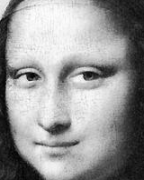
\includegraphics[width=0.4\textwidth]{images/eigenfaces/mona_lisa_original}
	\end{minipage}
\end{losung*}
Wir haben die Eigengesichter einfach als eine spezielle orthonormale Basis des Raumes der Differenzgesichter eingeführt.
Tatsächlich sind sie aber nicht etwa eine fixe Basis, sonder sie werden aus den Bilder der Datenbank berechnet.
Insbesondere erhält man mit einer anderen Datenbank auch andere Eigengesichter.
Aber wie diese Berechnung das genau geht, sehen wir später.
Zuerst wollen wir einige Eigenschaften dieser Basis untersuchen.